\chapter{Technology of ice stupas}
\label{chap:tech}

\cleanchapterquote{In building ice stupas, it's necessary to engage enough workforce to extract the water over
  long distances and to keep water flowing in cold temperatures.}{Marcus Nüsser}{(Professor, South Asia Institute)}

The tools used for ice stupa construction are limiting the water storage potential of this technology. The
fountain nozzle design is crucial for increasing the ice volumes achieved. However, no methodology currently
exists to rank the several fountain nozzles used for construction. An ideal pipeline configuration could make
this technology cheaper and maintenance free. However, optimization of the pipeline material and diameters are
yet to be carried out despite the loss of human hours on pipeline freezing events and the potential cost
reduction possible through use of cheaper pipeline materials and sizes. Water supply management based on
real-time weather conditions can dramatically improve water-use efficiency. However, constant water supply is
provided for fountain operation despite the significant diurnal and seasonal variation of weather conditions.

\section{Fountain scheduling strategies for AIR water supply management}

Among the above optimization issues, water supply management is the only one where the methodologies developed
in this thesis can be applicable. Water supply management can be achieved through fountain scheduling. Fountain
scheduling is simply answering the questions of “When do we spray?”, “How much do we spray?” and “How long do we
spray?”. Starting a fountain spray too early, spraying too much water or running a fountain spray too long might
lead to overwatering. At the very least, this practice wastes water.  Similarly, starting the fountain spray too
late, spraying too little water or not running the system long enough might lead to underwatering and can cause
reduced ice volumes or freezing of water supply pipelines.

Paper I has shown that traditional construction systems suffer from overwatering. In order to avoid this issue,
it is important to understand surface freezing rates, which can be calculated by means of the full energy
balance model developed in the last chapter.

There are some practical issues that need to be addressed before dealing with the fountain scheduling processes.
For example, in the case of the Indian AIR, the fountain discharge rate could have been halved since they were
always two times higher than the modelled freezing rate (paper I). However, in practice, reduction of discharge
rate could increase the maintenance cost due to higher risk of freezing events in the fountain pipeline.

An optimum construction strategy, therefore, should first prevent the occurrence of freezing events in the
fountain pipeline. These events can be prevented by setting a minimum threshold for the recommended discharge
rate. Additionally, recommended discharge rate needs to be sensitive to constraints on the water supply or
weather of the construction site. For example, locations limited by their water supply like Ladakh, India
would prioritize water use efficiency whereas those limited by the duration of their favourable weather windows
like Guttannen, Switzerland would prioritize maximum ice volume. The discharge scheduler software developed in
the previous chapter satisifies these requirements.

However, manually adjusting the fountain discharge rate is not practical due to two reasons- Firstly, this would
involve constant adjustments of discharge rates in response to the significant diurnal and seasonal variations
of the freezing rates. Secondly, frequent pipeline water drainage is required to avoid water losses. Therefore,
operation of scheduled fountains via automation systems is preferred to reduce the long-term maintenance costs.

The specific objectives of this study are to compare the water-use efficiency, maximum ice volume and
maintenance effort between traditional and automated construction strategies. In a first step, two AIRs were
built in the same location but with and without automated fountain scheduling strategies were measured and
compared. In a second step, the differences between these two construction strategies among Indian and Swiss
AIRs studied in previous winters were quantified using model simulations. 

\begin{figure}[htb]
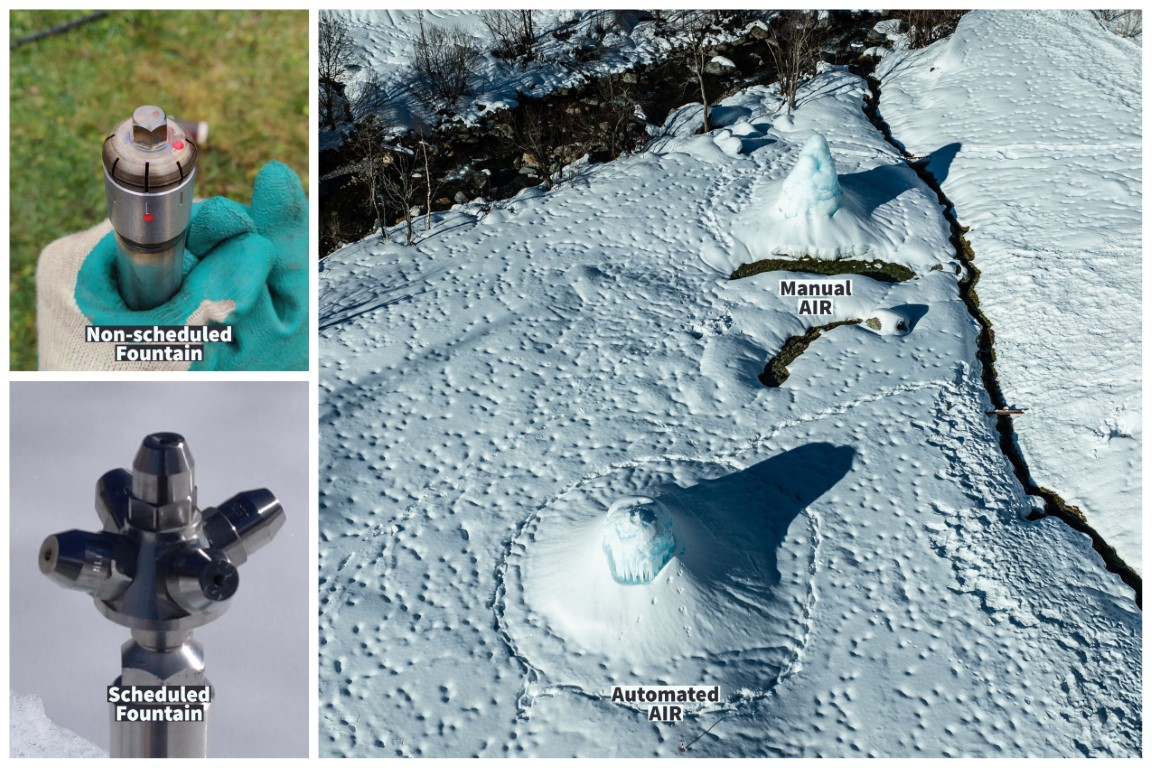
\includegraphics[width=12cm]{figs/AIR_fountains.jpg}
\caption{Unscheduled and scheduled fountains used for construction of traditional and automated AIRs at Guttannen. Picture credits: Daniel Bürki}
\label{fig:2AIR}
\end{figure}

\begin{figure}[htb]
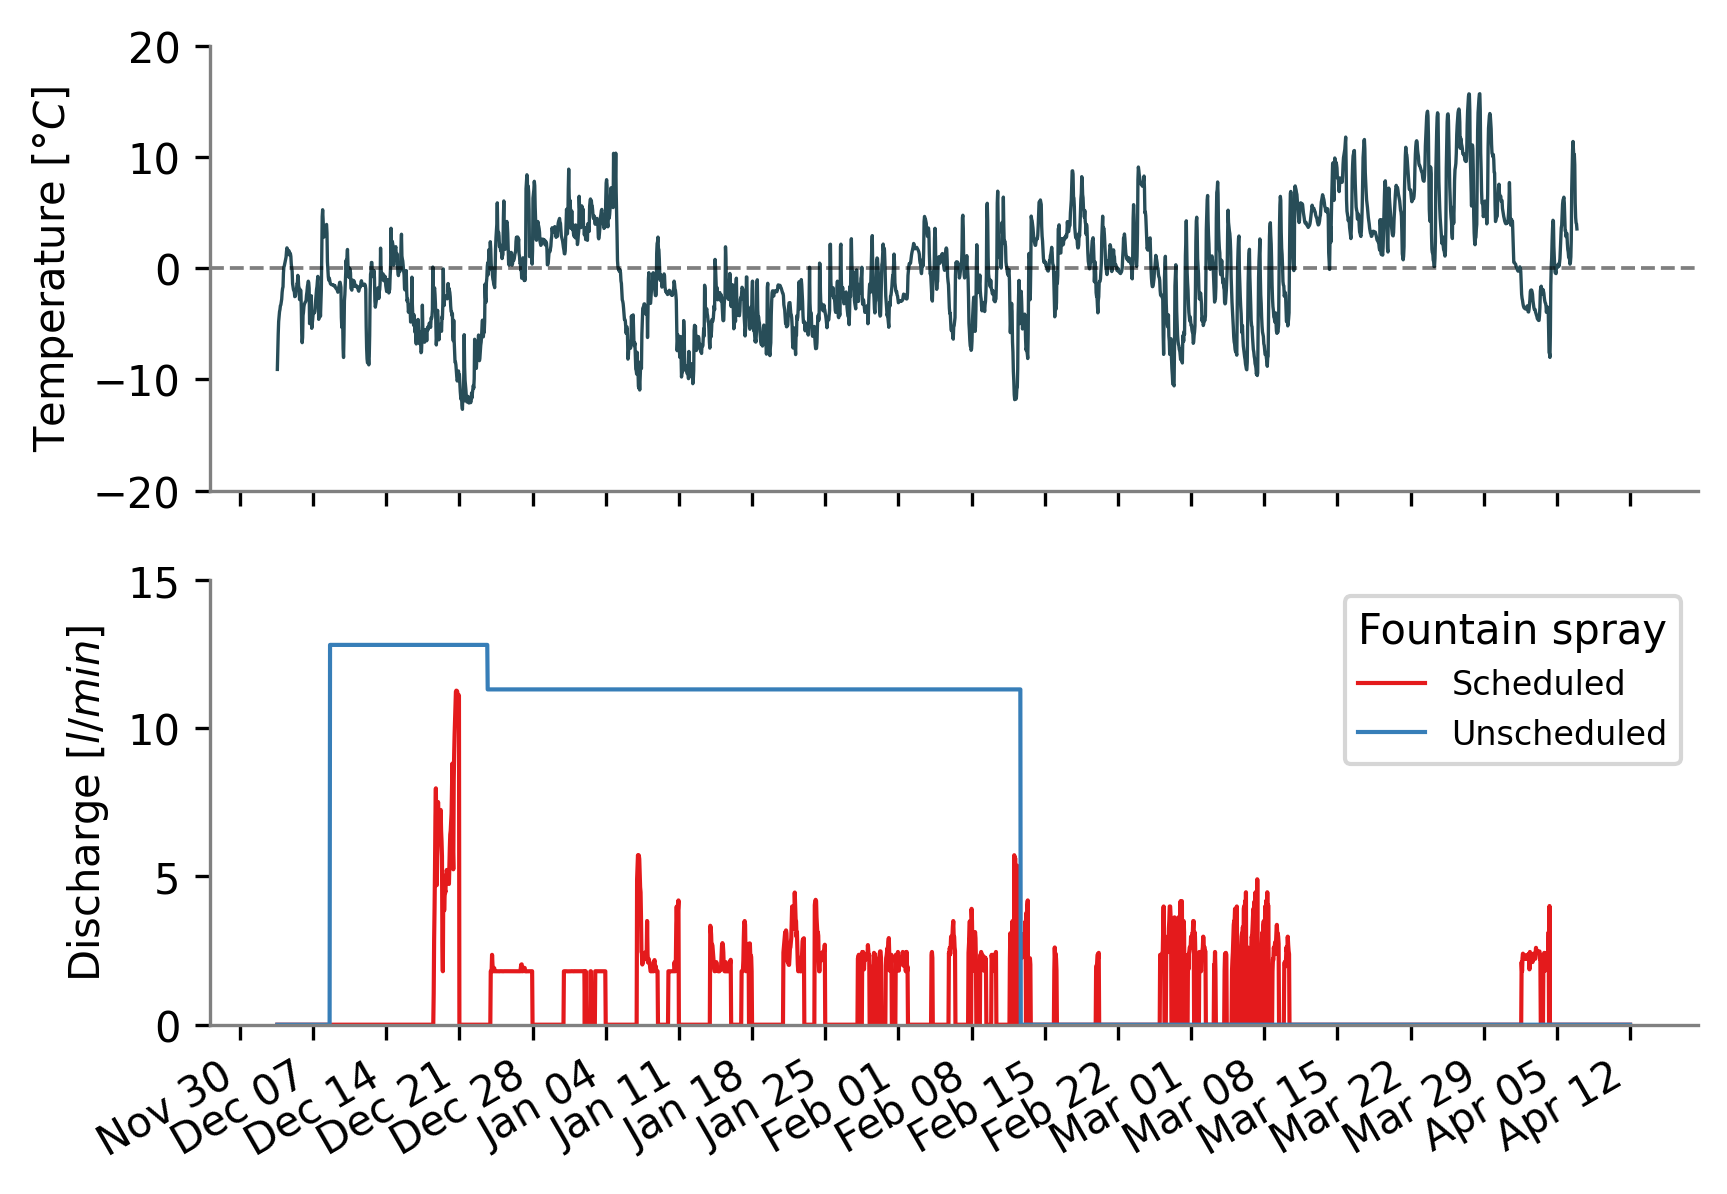
\includegraphics[width=12cm]{figs/disvstemp.png}
\caption{Temperature and discharge measurements of the two fountains at the Guttannen construction site.}
\label{fig:disvstemp}
\end{figure}

\begin{figure}[htb]
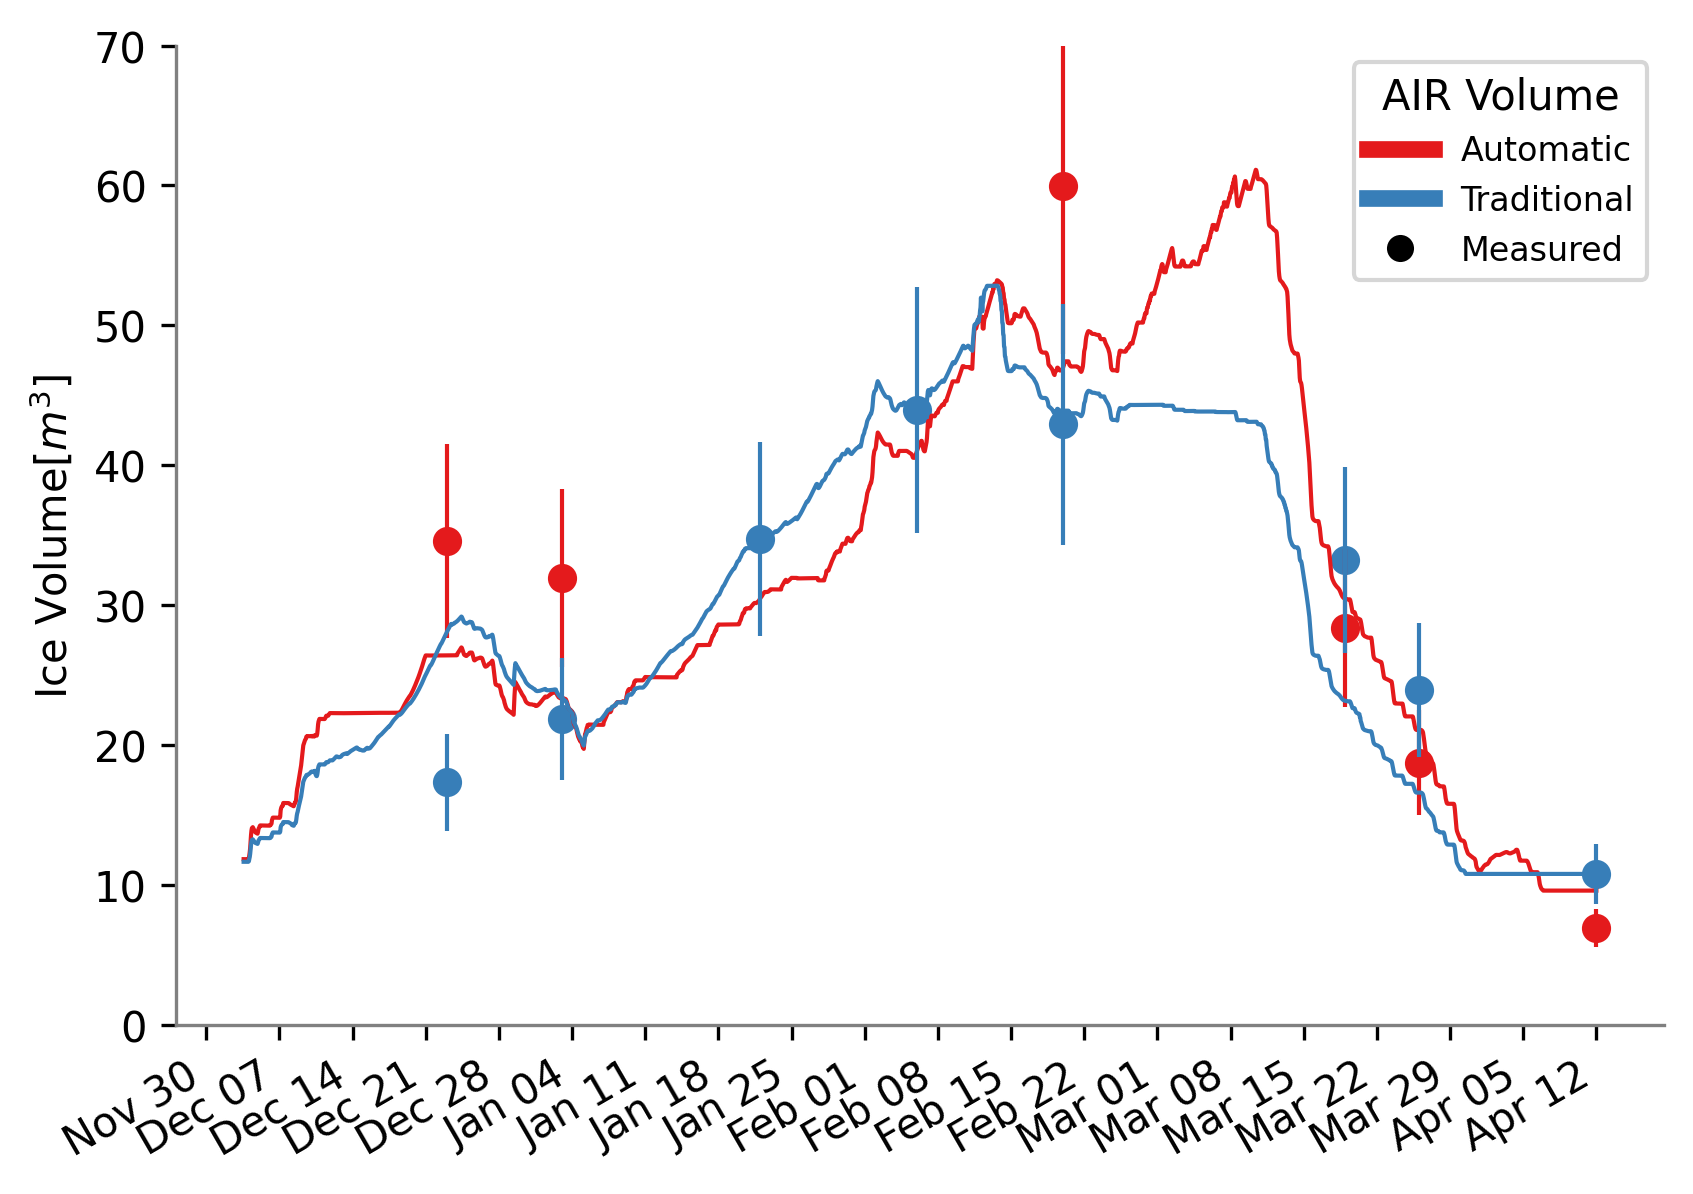
\includegraphics[width=12cm]{figs/auto_validation.png}
\caption{Volume validation of the scheduled and unscheduled fountain construction strategies.} 
\label{fig:auto_validation} \end{figure}

\subsection{Benefits of fountain scheduling}

The two AIRs built using a traditional and automated construction strategy are shown in Fig. \ref{fig:2AIR}. We
found that overwatering by unscheduled fountains not just increased the fountain wastewater production but also
enhanced the melting rate of AIRs, mainly due to its surface albedo and fountain heat flux feedbacks. Scheduled
fountains, in contrast, consumed only 13 \% of the unscheduled fountain's water supply. However, the volume
evolution of both the AIRs showed no significant variations. 

\begin{figure*}[htb]
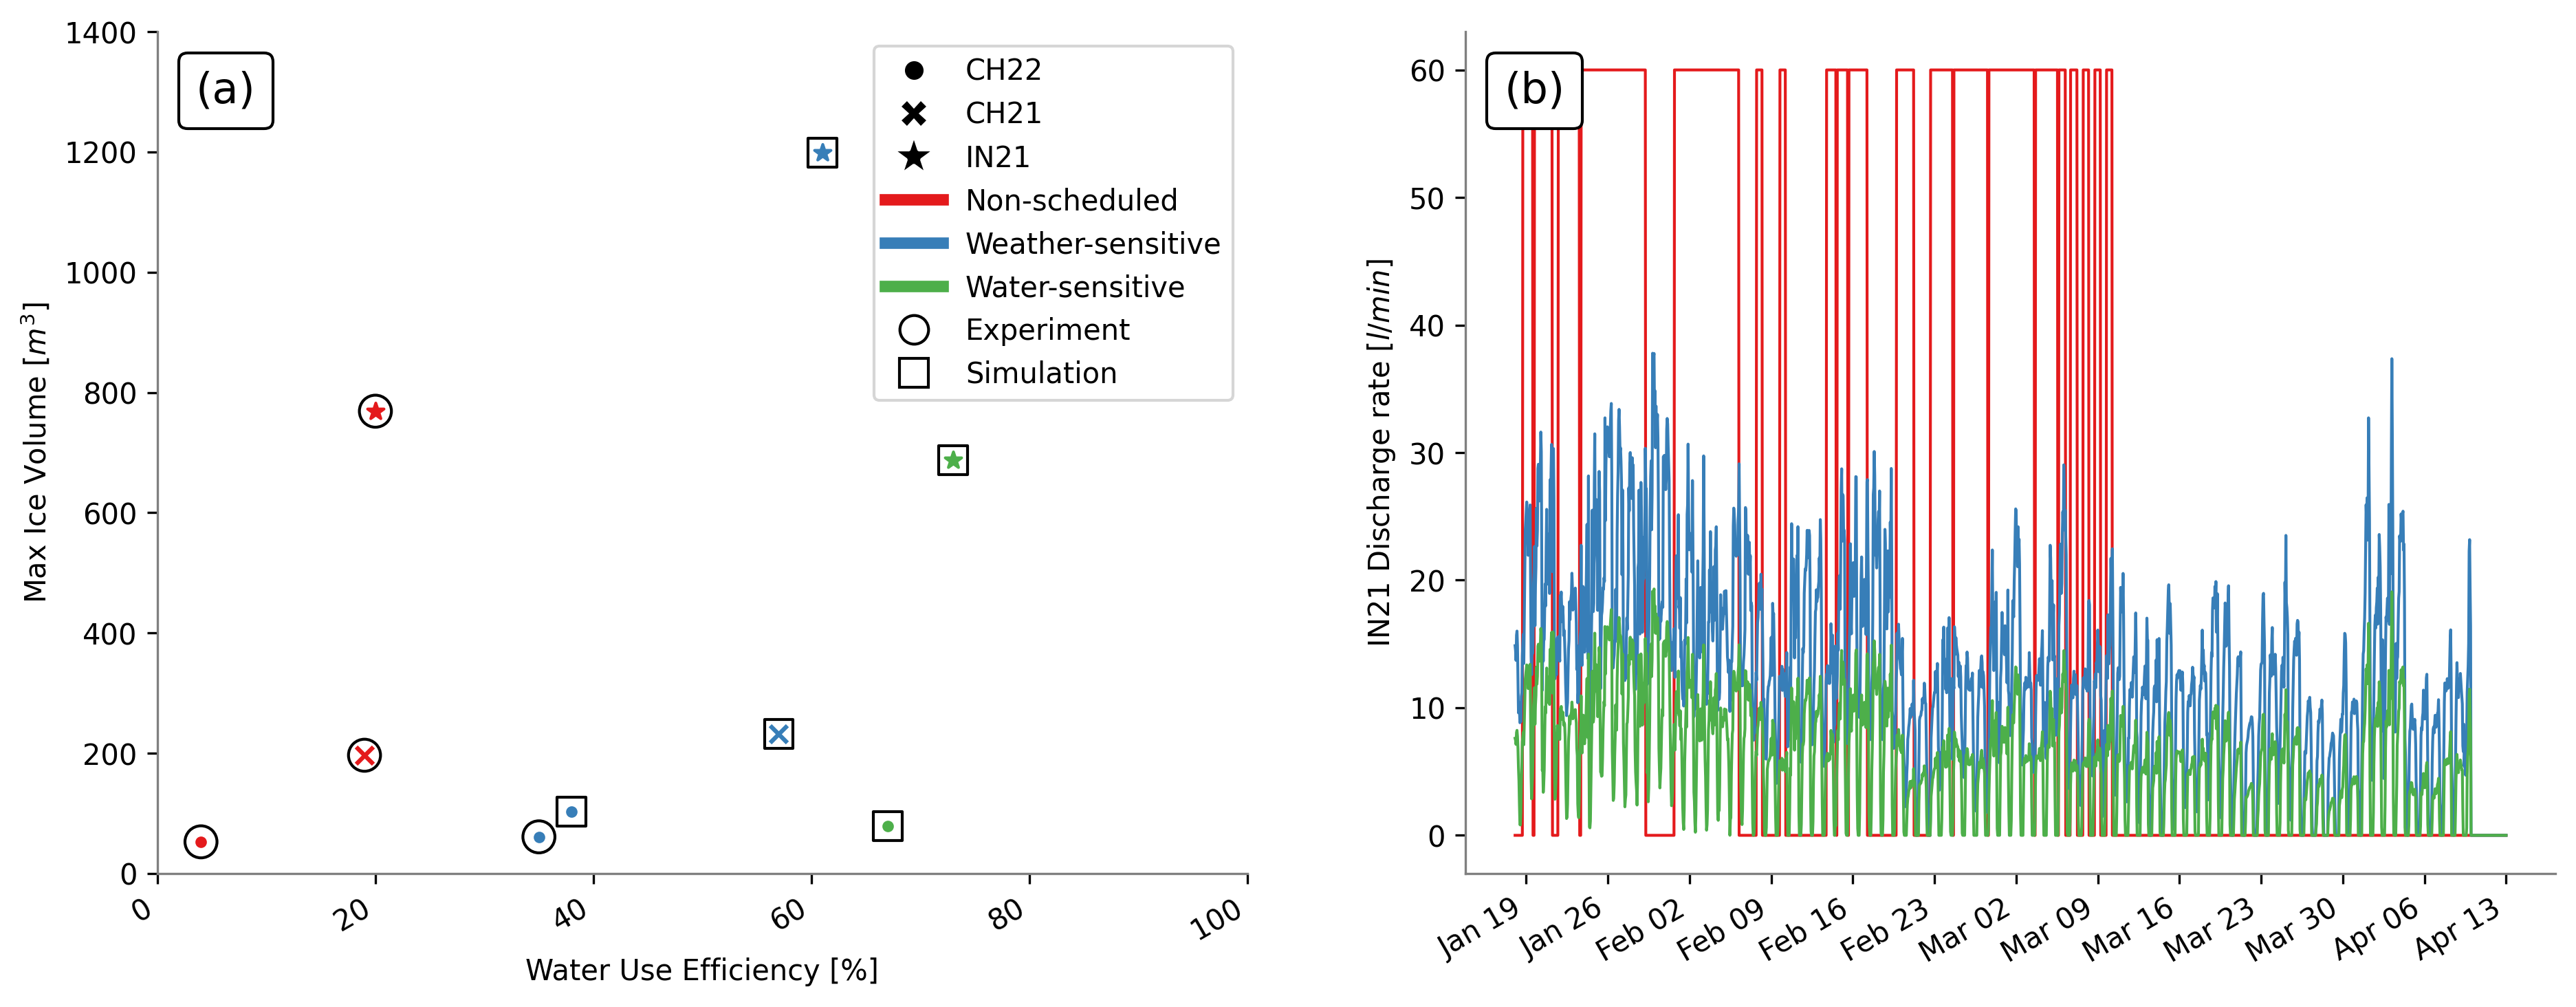
\includegraphics[width=\textwidth]{figs/wue.png}

\caption{(a) The maximum volumes and water-use efficiency estimated for AIRs constructed in different locations
(represented by colours) with different fountain scheduling strategies (represented by symbols). Experimental
values are highlighted by circles and simulated values are highlighted by squares. (b) Comparison of
the unscheduled and scheduled fountain's discharge rates at the IN21 location.}

\label{fig:wue}
\end{figure*}

The difference in water-use efficiency and maximum ice volume between unscheduled and scheduled fountains in the two
locations across two winters are presented in Fig. \ref{fig:wue} (a). Four experimental values (highlighted by
circles) are shown together with five simulated values (highlighted by squares).  The experimental values were
taken from the IN21 and CH21 AIRs studied in paper I and
the CH22 AIRs presented in paper II. 

The water-use efficiency of all the unscheduled fountains are below 20 \%. In general, the water-use efficiency
increases more than three folds when the weather-sensitive or water-sensitive fountains are used in both
locations.  

For the Indian location, the three kinds of fountains yield significantly different results.  The discharge
duration and the max discharge rate of the three IN21 fountains were responsible for these different results
(see Fig. \ref{fig:wue} (b)). The max discharge rate of the unscheduled fountain was more than twice that of
scheduled fountains resulting in a higher water loss. Freezing events in the fountain pipeline caused frequent
interruptions in the unscheduled discharge rate (see Fig. \ref{fig:wue} (b)). In contrast, the mean freezing
rates of the other two fountains during these events were above their median values. This is because, very cold
temperatures freeze the water inside rather than outside the fountain system instigating these freezing events in
the fountain pipeline. Therefore, both the discharge duration and the mean freezing rate of the unscheduled
fountain was much lower resulting in lower ice volumes. The water-sensitive fountain underestimated the freezing
rate during the construction period and therefore produced much lower ice volumes compared to the
weather-sensitive fountain. 

For the Swiss locations, scheduled fountains yielded better water-use efficiency but did not alter the maximum
volume obtained significantly. 


\section{Discussion}
\subsection{Ice stupas vs Ice terraces}

\begin{table}[htb]
	\begin{tabularx}{\textwidth}{X | X | X | X}
		\hline
    \textbf{Technology}& \textbf{Water storage}& \textbf{Daily meltwater supply (days)}& \textbf{Duration} \\
    \hline
		Ice terraces			& < 30				     & 2 months				\\
    Ice stupas        & < 10             & 5				\\
		\hline
	\end{tabularx}
	\label{tab:table1}
	\caption{This is a caption text.}
\end{table}

\subsection{Artificial glaciers: A thought experiment}

By definition, all glaciers, including the smallest ones, are bodies of sedimentary ice which were built up by
progressive snow compaction and firnification and flow downhill under the influence of gravity
\cite{benndouglasiGlaciersGlaciation2014}. Hence, because of their genesis and composition, AIRs differ from
glaciers. But when classified in terms of size and survival duration, AIRs exhibit similar characterestics to
very small glaciers. The glossary of glacier mass balance and related terms by
\citet{cogleyGlossaryGlacierMass2010} defines very small glaciers or glacierets as follows:

\begin{thesis_quotation}
  A very small glacier, typically less than 0.25 $km^2$ in extent, with no marked flow pattern
  visible at the surface. To qualify as a glacieret, an ice body must persist for at least two consecutive
  years. Glacierets can be of any shape, and usually occupy sheltered parts of the landscape. Windborne snow and
  avalanches can be dominant contributors to the accumulation of glacierets. 
\end{thesis_quotation}

This rather broad definition of glacierets or very small glaciers may be the one best suited for AIRs. Ice
terraces have been measured to have areas upto 0.15 $km^2$ by
\citet{nusserSociohydrologyArtificialGlaciers2019}. Ice stupas have been observed to last for two consecutive
years. However, most AIRs are neither so large or last so long.

Based on this definition, we can define "artificial glaciers" as ice bodies that are both larger in area and
last longer than two consecutive years. Manmade ice structures can, in theory, occupy any area provided for
their construction. But can AIRs, like glaciers, also survive the summer and compound their size every
consecutive winter? 

\begin{figure}[htb]
  \centering
	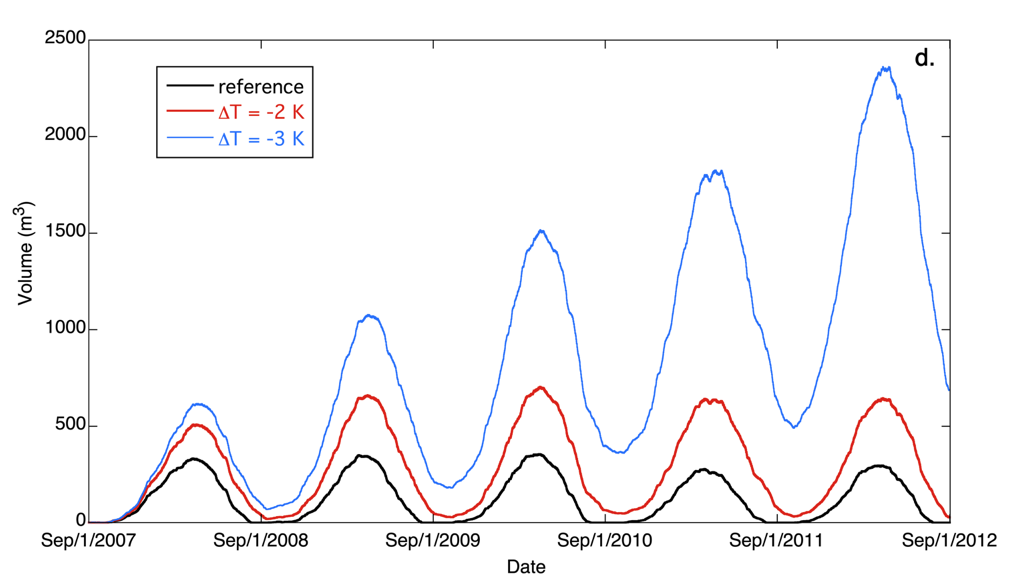
\includegraphics[width=12 cm]{figs/PIR_example.png}
  \caption{The effect of a negative temperature perturbation. For $\Delta T = -3 \degree C$ the icestupa does
  not disappear anymore but is growing from year to year.}
\label{fig:PIR}
\end{figure}

A possible way to study this question is to decrease the air temperature uniformly (temperature change $\Delta
T$). This will imply a stronger negative sensible heat flux in summer, thus accelerating icestupa growth and
slowing down its decay. We found a break-even point for $\Delta T = -2 \degree C$ (Fig. \ref{fig:PIR}). For
larger negative values of $\Delta T$ the icestupa does not disappear in summer and keeps growing from year to
year. For $\Delta T = -3 \degree C$, the maximum volume in the fifth year is about 4 times that in the first
year. Therefore, there exists weather conditions where they can last as long as the water supplies last (see
Fig. \ref{fig:PIR}). Paper III provides the datasets and methodology used to produce these simulations.



% \subsection{Suggested improvement of construction tools}

% \subsubsection{Pipeline configuration}

% The typical pipeline configuration in Ladakh is prone to pipeline freezing events. Therefore, the pipeline
% material with higher insulation properties and diameter is required to lower this risk. Further effort is needed
% to find a cost effective way to achieve an ideal pipeline configuration.

% \subsubsection{Fountain nozzle}

% Even though several AIR fountain nozzles exist, there does not exist a strategy to choose the best among them.
% Their efficacy is expected to increase with lower droplet sizes, higher flight times and higher spray radius.
% Therefore, a comparative study of all the AIR fountain nozzles used across these four factors would help make an
% informed choice for future AIR constructions.

% \subsubsection{Water supply management}

% All the studied AIRs suffer from overwatering (paper I). Automated fountain water supply management has been
% shown to increase their water use efficiency of AIRs and reduce their maintenance without compromising on their
% meltwater production. The methodology to implement this new construction strategy is presented in paper II.

% AIRs are a natural evolution of Ladakh's agricultural system. They can be related to traditional water
% harvesting technologies like the \textit{zing}, which are small tanks where meltwater is collected through the use
% of an intricate network of channels. The mountain oases of the Hindu Kush and Karakoram ranges
% have similar irrigation networks \citep{nusserLocalKnowledgeGlobal2016}.

% Ice terraces are the oldest form of AIRs \citep{norphelArtificialGlacierHigh2009}. Usually situated below the
% glaciers at elevations where snowmelt starts end of March, these structures facilitate the freezing of stream
% water during winter at selected sites, usually shaded by surrounding mountains. 

% \subsection{Ice terraces}

% \begin{figure}[t]
% \centering
% 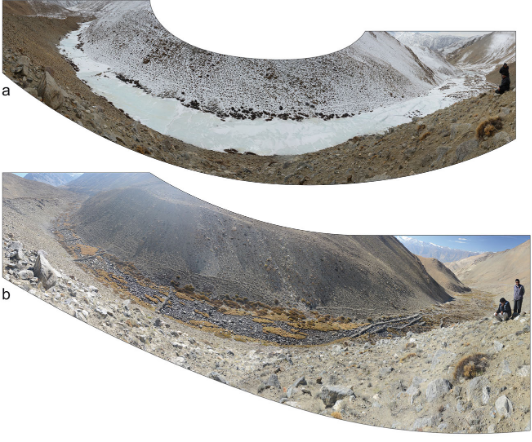
\includegraphics[width=12cm]{figs/IT_example.png}

% \caption{Ice terrace of Phuktse, viewpoint 4430 m. (a) February 2014 (b) October 2014 Adapted from: \cite{nusserSociohydrologyArtificialGlaciers2019}}

% \label{fig:ITexample}
% \end{figure}

% According to oral history and Corona imagery from 1969, the first ice terraces are older than 50 years and can
% be found in Phuktse and Igoo. Over the past 30 years, 14 ice terraces have been constructed in central Ladakh,
% located in tributary valleys of the Indus \citep{norphelArtificialGlacierHigh2009,
% nusserSociohydrologyArtificialGlaciers2019}. Chewang Norphel, a well known engineer of the Leh Nutrition
% Project, introduced this practice to Ladakh \citep{vinceGlacierMan2009}. Cascades and diversions shown in Fig.
% \ref{fig:AIRdesigns} constitute the ice terrace type of AIRs due to their shape. In February 2014, Phuktse built
% a successful cascade with an almost continuous stretch of ice (Fig. \ref{fig:ITexample}). 

% \subsubsection{Traditional construction strategy}

% There are two distinct types of ice terraces with site-specific modifications as shown in Fig.
% \ref{fig:AIRdesigns}: the first type is built as cascades on perennial streams. A series of loose rock walls in
% the river bed reduces flow velocity, but still lets water pass through. Such cascades allow flowing water to
% freeze on exposed surfaces and form superimposed ice layers when temperatures drop (see Fig.
% \ref{fig:ITscience}). 

% The second type diverts water from streams with higher flow velocity to small side valleys, shaded by
% surrounding mountains. This design allows to integrate higher slope positions for additional ice formation. It
% consists of a series of partially cemented stone walls across the stream bed. Their dimensions are adjusted
% based on the valley topography. The water for the ice terrace is obtained through a long diversion channel. 

% \begin{figure}[htb]
% \centering
% 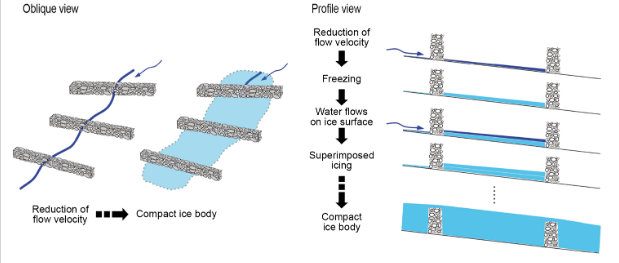
\includegraphics[width=12cm]{figs/IT_science.png}

% \caption{ The process of ice accumulation for ice terraces Adapted from:
% \cite{nusserSociohydrologyArtificialGlaciers2019}}

% \label{fig:ITscience}
% \end{figure}

% As mentioned in the previous chapter, the design of the ice terraces is dependent on the suitability of the
% site. Furthermore, the following construction guidelines are used depending on the terrain of the site
% \cite{norphelSnowWaterHarvesting2015}:

% \begin{itemize}

%   \item If the section of the stream is very wide with a mild slope, then the stone walls are
%     constructed in a series parallel to each other. The number and dimension of ice retaining walls depend on
%     the flow of water available in the main stream during peak winter. In November, when winter begins, some
%     locally available wild grass is put on the base of the dry bund to plug any holes.

%   \item If the section of the stream is narrow with a steep grade then it needs to be diverted to a shady area
%     by constructing a gravitational channel with a slope of 1:30. When it reaches the ice terrace site the slope
%     should be gradually reduced to 1:50, allowing it to flow through small outlets to accelerate freezing. Stone
%     walls need to be constructed parallel to the channel in series at a distance of 10-30 m, accoring to the
%     natural slope of terrain. The steeper the terrain, the smaller the distance and slope between the bunds.

% \end{itemize}

% \subsubsection{Water storage and cost}

% Ice volume variations of different ice terraces within Ladakh \citep{nusserSociohydrologyArtificialGlaciers2019,
% norphelSnowWaterHarvesting2015} range from 510 $m^3$ to 81,040 $m^3$ highlighting the importance of local topography and
% microclimate in their formation. The cost of construction depends on the size and number of stone walls
% required. The estimated cost of ice terraces vary between 4600 to 15,330 USD
% \cite{nusserSociohydrologyArtificialGlaciers2019}. The location requirements and the construction cost of ice
% terraces, therefore, were prohibitive for widespread adoption.

% \subsection{Ice stupas}

% \begin{figure}[htb]
% \centering
% 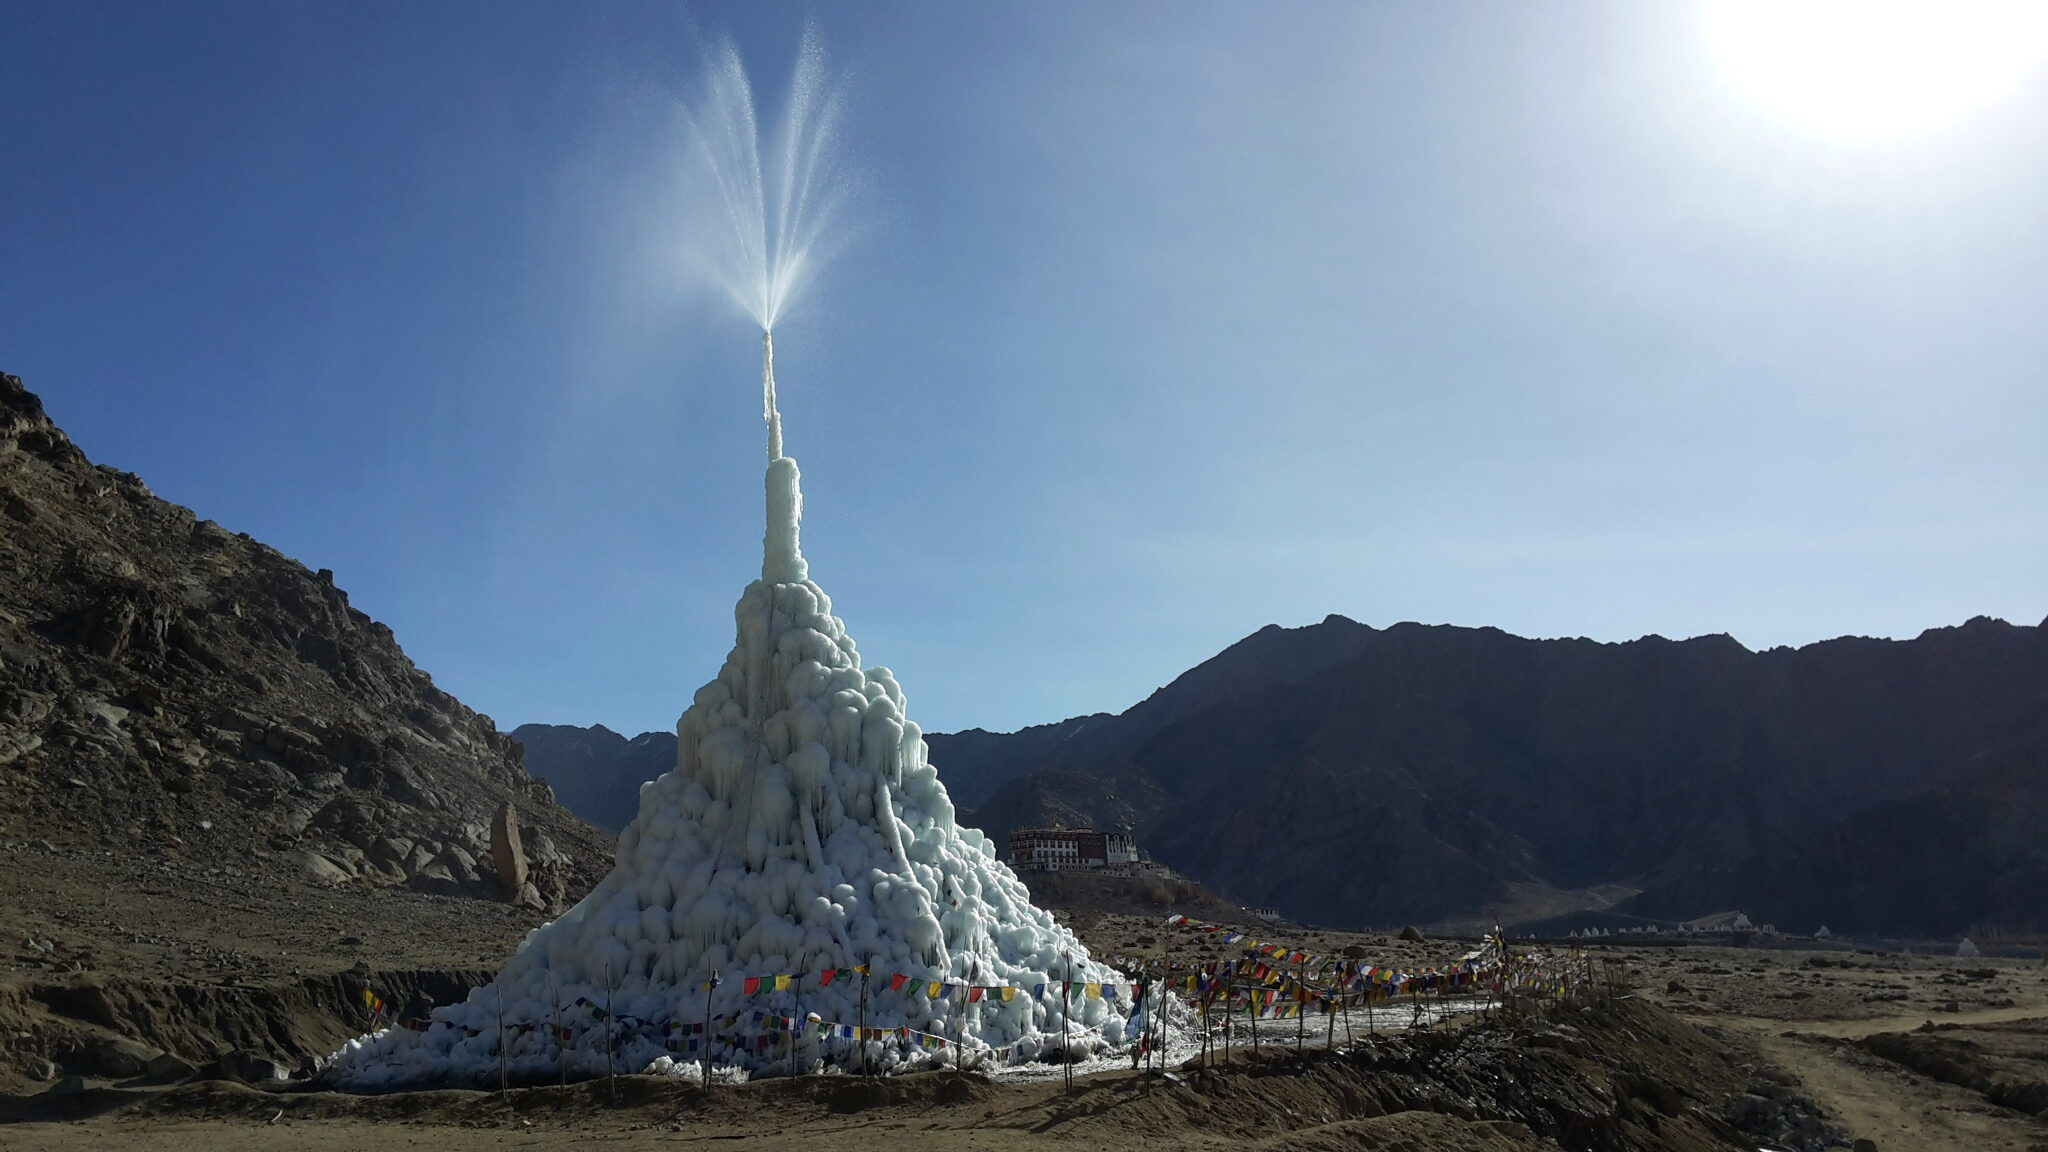
\includegraphics[width=12cm]{figs/IS_example.jpg}

% \caption{Ice stupa of Shara}

% \label{fig:ISexample}
% \end{figure}

% Ice stupas were invented by Sonam Wangchuk in 2013 \cite{wangchukIceStupaArtificial2014} to provide a much
% cheaper alternative to achieve water storage compared to ice terraces. Ice stupas can also be placed much closer
% to the plantations since they absorb lesser solar radiation per unit volume compared to ice terraces due to
% their conical shape. However, the typical volume range of ice stupas (see Fig. \ref{fig:airs_ladakh}) are also
% much smaller than ice terraces. Over the past decade, several ice stupas have been built to supplement
% irrigation water supply of mountain villages in India \citep{wangchukIceStupaCompetition2020,
% palmerStoringFrozenWater2022, aggarwalAdaptationClimateChange2021}, Kyrgyzstan
% \citep{bbcnewsBrightArtificialGlacier2020} and Chile \citep{reutersConservationistsChileAim2021}. 

% \subsubsection{Traditional construction strategy}

% \begin{figure}[htb]
% \centering
% 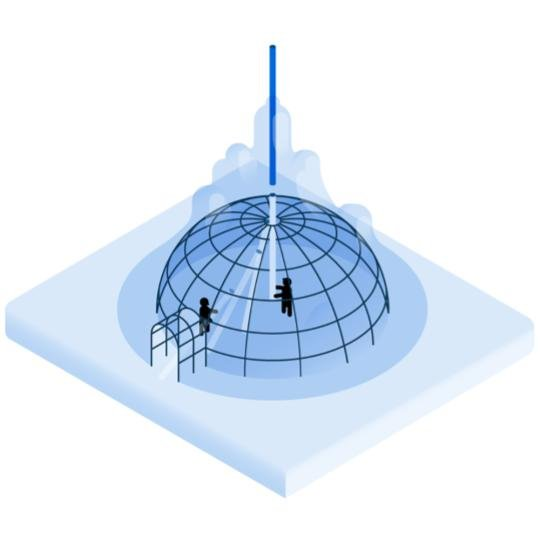
\includegraphics[width=8cm]{figs/IS_science.jpg}

% \caption{The construction process of ice stupas. Diagrams by: Francesco Muzzi }

% \label{fig:ISconstruction}
% \end{figure}

% A typical AIR (see Fig. \ref{fig:ISexample}) simply requires a fountain nozzle mounted on a supply pipeline. The
% water source is usually a glacial stream. Due to the altitude difference between the pipeline input and fountain
% output, water ejects from the fountain nozzle as droplets which freeze under subzero winter conditions. The
% fountain is manually activated during winter nights. The fountain nozzle is raised through the addition of metal
% pipes when significant ice accumulates below (see Fig. \ref{fig:ISconstruction}).  Typically, a dome of branches
% is constructed around the metal pipes so that pipe extensions can be done from within this dome. Threads, tree
% branches and fishing nets are used to guide and accelerate the ice formation.

% \subsubsection{Water storage and cost}

% \begin{figure}[htb]
% \centering
% 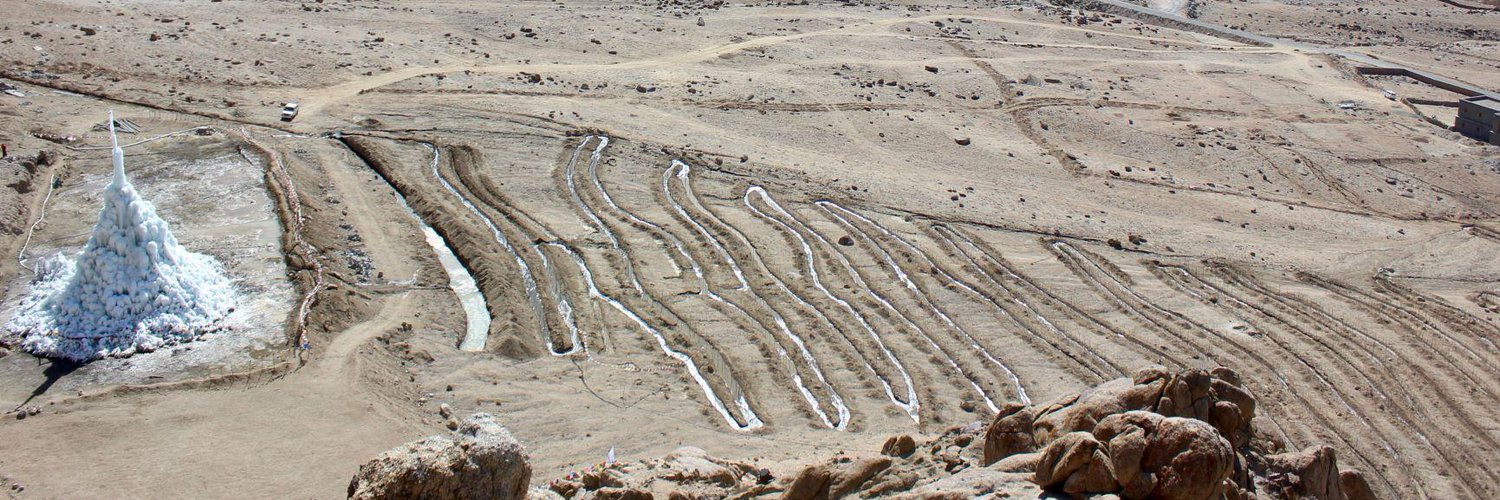
\includegraphics[width=12cm]{figs/IS_irrigation.jpeg}

% \caption{Irrigation channel of the IN17 and IN18 AIRs. (P.C. Lobzang Dadul) }

% \label{fig:ISirrigation}
% \end{figure}

% \begin{figure}[htb]
% \centering
% 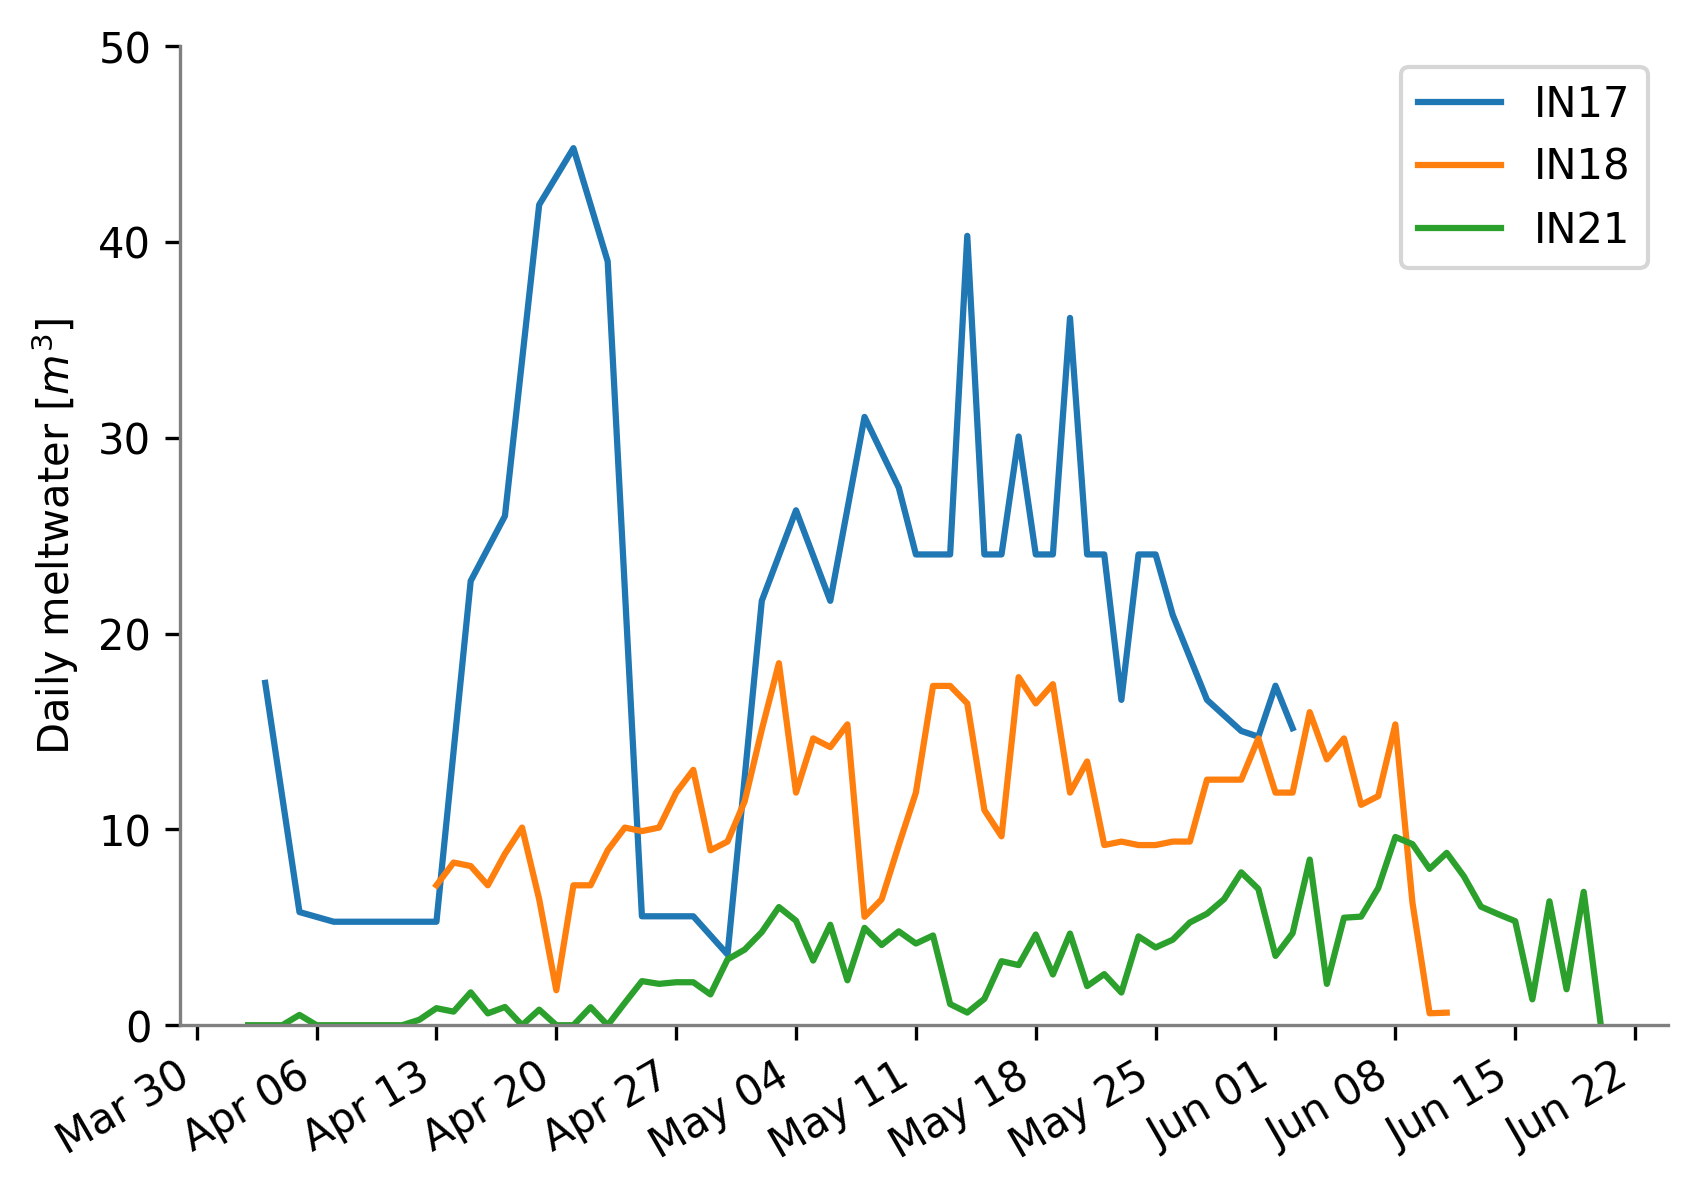
\includegraphics[width=12cm]{figs/melt.png}

% \caption{Daily meltwater measurements for the IN17 and IN18 AIRs along with the corresponding model estimations
% for the IN21 AIR. }

% \label{fig:ISmelt}
% \end{figure}

% The cost of construction primarily depends on the material, size and length of the pipeline required. The
% fountain nozzle cost is negligible in comparison. Typical pipeline configuration in Ladakh consists of a high
% density polyethylene pipeline of 60 mm diameter and upto 5 km in length and 60 m of head. The estimated cost
% of ice stupas vary between USD.

% Fig. \ref{fig:ISmelt} shows the temporal variation of daily meltwater quantities obtained from 3 different AIRs
% built in Ladakh during their melting periods (mid-April to mid-June). IN17 and IN18 AIRs were constructed in
% Phyang village and their meltwater quantities was measured manually using the storage tank shown in Fig.
% \ref{fig:ISirrigation}. The details of this measurement strategy are presented in Appendix. IN21 was constructed
% in Gangles village and its meltwater quantities were modelled. The differences between the AIRs reflect the
% corresponding interannual variability in the weather conditions. The average median daily AIR meltwater
% quantities during these 3 melting seasons was around 12 million litres.    

% There is no, and probably will never be, consensus about how to define AIRs. Therefore, no conclusive definition
% of AIRs is promoted in this thesis, either.
% The rise of ice harvesting technologies has pushed the boundaries of the size and survival duration of manmade
% ice structures.
